%% LaTeX-Beamer poster template for KIT design
%% by Erik Burger, Christian Hammer
%%
%% version 1.2
%%
%% mostly compatible to KIT corporate design v1.2
%% http://www.uni-karlsruhe.de/download/uka/Gestaltungsrichtlinien_komplett.pdf
%%
%% Problems, bugs and comments to
%% burger@kit.edu

\documentclass{beamer}

%% Fill in the page size here. If the proportions of the fonts
%% are not satisfactory, change the scale parameter
\usepackage[orientation=portrait,size=a0,scale=1.4]{beamerposter}
\usepackage[utf8]{inputenc}

\mode<presentation>{\usetheme{kitposter}}

\title[gr-inspector]{The Inspector (gr-inspector)}
\subtitle{A Signal Analysis Toolbox for GNU Radio}
\author{Sebastian Müller, Karlsruhe Institute of Technology (gsenpo@gmail.com)}

\institute{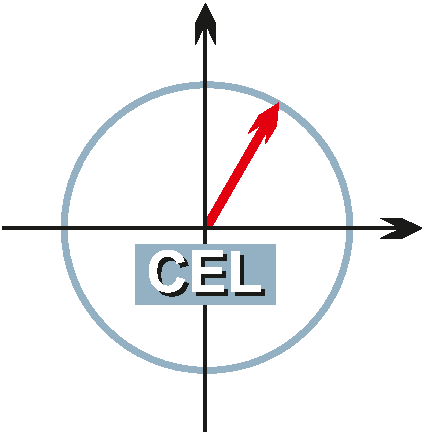
\includegraphics[height=250px]{logos/cel.pdf}\textbf{Communications Engineering Lab}\\[.4em]
Kreuzstr. 11\\[.2em]
76137 Karlsruhe\\[.4em]
\href{http://www.cel.kit.edu}{http://www.cel.kit.edu}}

\begin{document}
% change the following line to "ngerman" for German style date and logos
\selectlanguage{english}

\begin{frame}
  \begin{columns}[t]
    \begin{column}{0.33\textwidth}
      \frametitle{Main}
      \begin{block}{Introduction}
        gr-inspector is an out-of-tree module for GNU Radio. The target was to develop a signal analysis toolbox with the following real-time capabilities:\\[0.5em]
        \begin{itemize}
	        \item Automatic signal detection
	        \item Automatic Signal Classification (AMC)
          \item OFDM parameter estimation and synchronization
	        \item GUI feedback
        \end{itemize}
        \vspace{0.5em}
        This project was part of Google Summer of Code and ESA Summer of Code in Space programs.
      \end{block}
      \begin{block}{Components}
\textbf{Signal Detector}
Is able to perform energy detection on an input signal.\\[0.5em]

\textbf{Inspector GUI}
The GUI block visualizes the detected signal edges. Users can select signals manually and feed analysis messages to be displayed in the GUI.\\[0.5em]

\textbf{Signal Separator}
Uses FIR filters for every detected/selected input signal to mix, filter and decimate this signal out of the input spectrum.\\[0.5em]

\textbf{Signal Extractor}
Passes one signal from the Separator output as complex stream. The input samples can be resampled to satisfy a constand output sample rate.\\[0.5em]

\textbf{AMC Block}
\textbf{TODO}\\[0.5em]

\textbf{OFDM Estimator}
Estimates OFDM parameters subcarrier spacing, symbol time, FFT lenght and CP length.\\[0.5em]

\textbf{OFDM Synchronizer}
After performed estimation, the signal can be frequency synchronized and stream tags can be inserted at OFDM symbol beginnings.
      \end{block}
    \end{column}
    \begin{column}{0.01\textwidth}
    \end{column}
    \begin{column}{0.66\textwidth}
      \begin{block}{Flowgraph}
        The toolbox was developed with the following main flowgraph in mind.
        \begin{figure}
          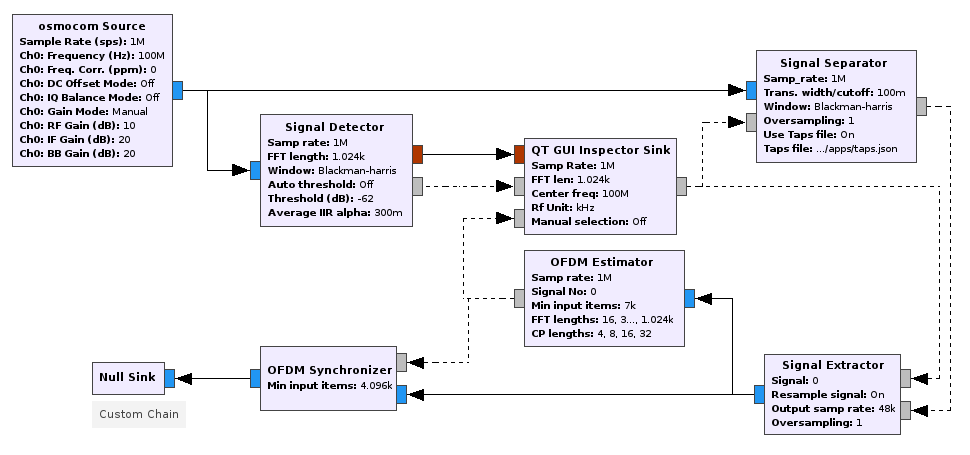
\includegraphics[width=\textwidth]{figures/flowgraph}
          \caption{Example flowgraph}
        \end{figure}

	      The \textbf{Signal Extractor} block assures the ability to append custom signal processing chains for users. Each analysis block can have a feedback message to the \textbf{Inspector GUI} to print their results there.
      \end{block}
      \begin{block}{GUI}
      \begin{figure}
      	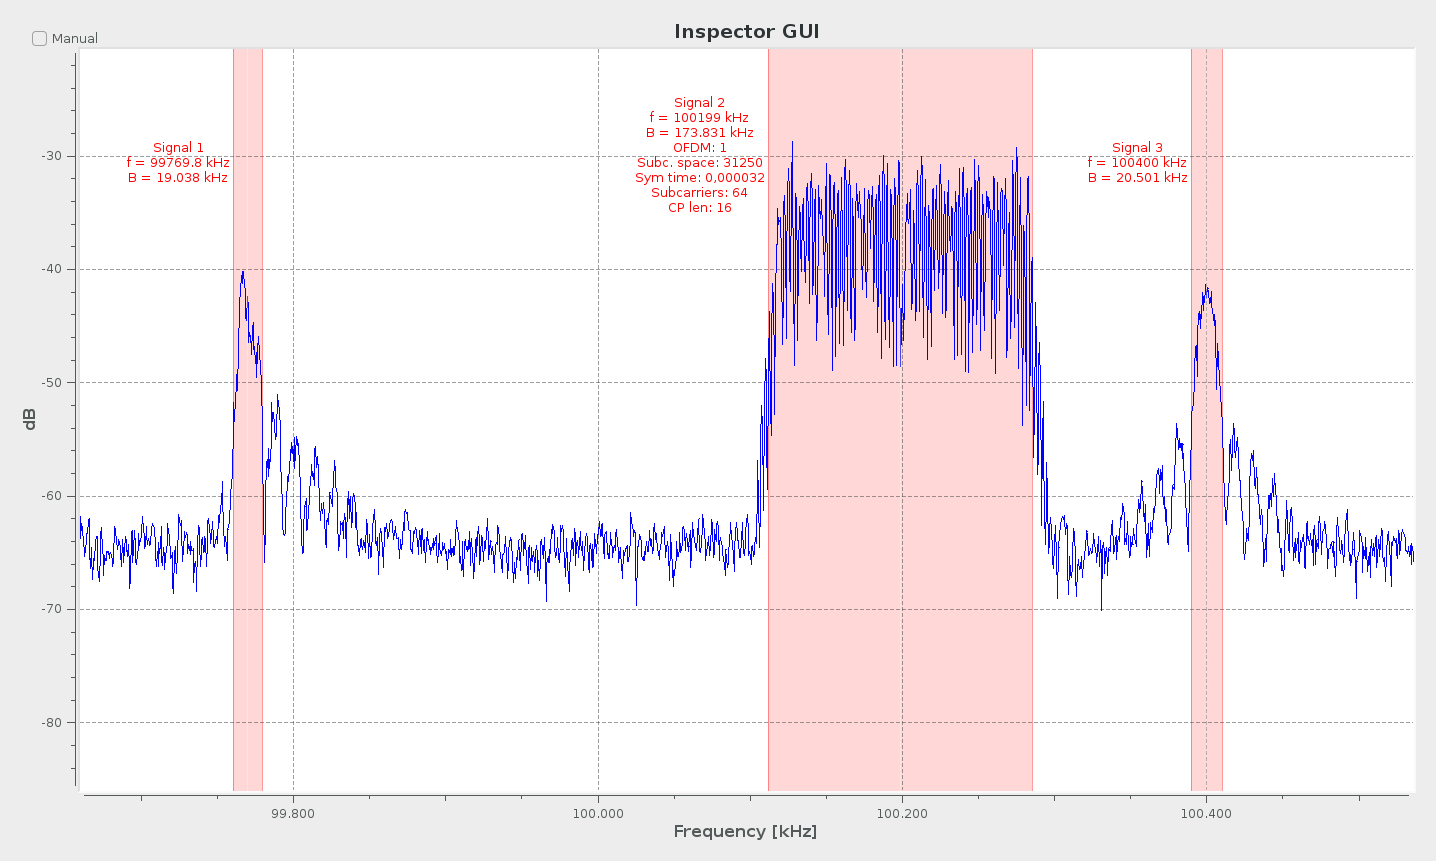
\includegraphics[width=\textwidth]{figures/gui.png}
      	\caption{Inspector GUI}
      \end{figure}
      	The GUI displays the input spectrum along with markers for all detected signals. Next to the graphical markers, information text is displayed. Each signal has a number and estimated \textbf{center frequency} and \textbf{bandwidth}. Distinct analysis toolboxes can provide \textbf{additional information} for specific signals, which will be appended to the info text.
      \end{block}
    \end{column}
  \end{columns}
  \begin{columns}[t]
  	\begin{column}{0.66\textwidth}
  		\begin{block}{References}
  			Some additional info
  		\end{block}
  	\end{column}
  	\begin{column}{0.01\textwidth}
  	\end{column}
  	\begin{column}{0.33\textwidth}
  		\begin{block}{Contact}
  			Maintainer of this module:\\~\\
  			Sebastian Müller

  			Karlsruhe Intitute of Technology

  			gsenpo@gmail.com
  		\end{block}
  	\end{column}
  \end{columns}
\end{frame}
\end{document}
